% !TEX TS-program = pdflatex
% !TEX encoding = UTF-8 Unicode

% This is a simple template for a LaTeX document using the "article" class.
% See "book", "report", "letter" for other types of document.

\documentclass[11pt]{article} % use larger type; default would be 10pt

\usepackage[utf8]{inputenc} % set input encoding (not needed with XeLaTeX)
\usepackage[english,swedish]{babel}
%%% Examples of Article customizations
% These packages are optional, depending whether you want the features they provide.
% See the LaTeX Companion or other references for full information.

%%% PAGE DIMENSIONS
\usepackage{geometry} % to change the page dimensions
\geometry{a4paper} % or letterpaper (US) or a5paper or....
% \geometry{margin=2in} % for example, change the margins to 2 inches all round
% \geometry{landscape} % set up the page for landscape
%   read geometry.pdf for detailed page layout information

\usepackage{graphicx} % support the \includegraphics command and options
\usepackage{datetime}
\usepackage{amssymb,amsmath} % For mathematical expressions  (Tillagd av Nai) 
\usepackage{textcomp} % For degree sign (Tillagd av Nai) 

%%% NEW COMMANDS
\renewcommand{\dateseparator}{-}
\newdateformat{mydate}{\THEYEAR \dateseparator0\THEMONTH \dateseparator \THEDAY} 
\renewcommand{\figurename}{Figur}

% \usepackage[parfill]{parskip} % Activate to begin paragraphs with an empty line rather than an indent

%%% PACKAGES
\usepackage{booktabs} % for much better looking tables
\usepackage{array} % for better arrays (eg matrices) in maths
\usepackage{paralist} % very flexible & customisable lists (eg. enumerate/itemize, etc.)
\usepackage{verbatim} % adds environment for commenting out blocks of text & for better verbatim
\usepackage{subfig} % make it possible to include more than one captioned figure/table in a single float
% These packages are all incorporated in the memoir class to one degree or another...

%%% HEADERS & FOOTERS
\usepackage{fancyhdr} % This should be set AFTER setting up the page geometry
\pagestyle{fancy} % options: empty , plain , fancy
\renewcommand{\headrulewidth}{0pt} % customise the layout...
\lhead{}\chead{}\rhead{}
\lfoot{}\cfoot{\thepage}\rfoot{}

%%% SECTION TITLE APPEARANCE
\usepackage{sectsty}
\allsectionsfont{\sffamily\mdseries\upshape} % (See the fntguide.pdf for font help)
% (This matches ConTeXt defaults)

%%% ToC (table of contents) APPEARANCE
\usepackage[nottoc,notlof,notlot]{tocbibind} % Put the bibliography in the ToC
\usepackage[titles,subfigure]{tocloft} % Alter the style of the Table of Contents
\renewcommand{\cftsecfont}{\rmfamily\mdseries\upshape}
\renewcommand{\cftsecpagefont}{\rmfamily\mdseries\upshape} % No bold!

\usepackage[font={small,it}]{caption} %change the caption of the images

%%% END Article customizations






%%% The "real" document content comes below...

\pagenumbering{gobble}
\title{Projektrapport Grupp 3 \\* 
Space Curling\\*
TNM085 Modelleringsprojekt}
\author{Linnéa Mellblom\\*Linnea Malcherek\\* Julia Nilsson\\*Michael Nilsson\\*Linnéa Nåbo}
%\date{} % Activate to display a given date or no date (if empty),
         % otherwise the current date is printed 
\mydate


\begin{document}
\maketitle
\pagebreak
\pagenumbering{arabic}  

\pagebreak
\tableofcontents
\pagebreak

\section{Introduktion}
Curling är ett intressant system att modellera eftersom det innefattar många vedertagna fysikaliska egenskaper men även delar som inte är särskilt triviala. 
De senaste åren har ett flertal vetenskapliga artiklar publicerats som ger sin förklaring till svängningsfenomenet, den så kallade "curlen", hos curlingstenen.
Gemensamt för artiklarna är hypotesen om att svängningen på curlingstenen beror på en högre friktion på bakre delen av stenen än den främre. 
Anledningen till varför det är så kommer att förklaras i denna rapport.

\begin{figure}[ht!]
\centering
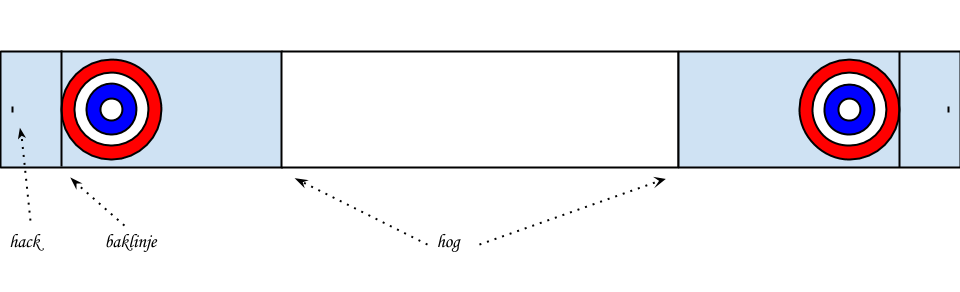
\includegraphics[width=140mm]{bana.png}
\caption{Curlingbanan}
\label{fig:bana}
\label{overflow}
\end{figure}

\subsection{Begränsningar och förenklingar} 
Denna rapport behandlar modellbygge och simulering av en curlingstens translation
och rotation, friktionens påverkan samt kollision mellan curlingstenar. 
Curlingstenarnai beräkningarna har samma massa och därmed kan beräkningar förenklas genom att
förkorta bort massan. I spelet använder man sig även av sopning för att påverka stenens
bana över isen. Det fungerar dock endast på den sten som senast skjutits ut. Hänsyn har
inte heller tagits till den rotation som skapas för stenarna efter en sned krock (krock som
inte är riktad mot masscentrum). Stenarna har istället samma rotationshastighet efter
krock som de hade innan.

\pagebreak

\section{Fysikalisk beskrivning} 

Alla variabler går att finna i en tabell i Apendix A.

\subsection{Translation}

I beräkningarna av stenens rörelse har hänsyn tagits till tre påverkande friktionskrafter (Figur~\ref{fig:Translation}): Kraft i riktning motsatt stenens rörelseriktning $\bar{F_f}$, samt två krafter i ortogonal riktning mot denna $\bar{F_1}$ och $\bar{F_2}$ \eqref{Ftot}. Dessa två krafter utgörs av friktionskrafterna i främre delen av stenen samt i den bakre delen. Differensen mellan dessa två krafter är vad som påverkar stenens curl (svängning). Summan av krafterna är den totala kraftpåverkan på stenen $\bar{F_t}$.

\begin{subequations}\label{Ftot}
 \begin{align}
 \bar{F_t}&=\bar{F_1}+\bar{F_2}+\bar{F_f}\\
 \bar{F_1}&<\bar{F_2}
 \end{align}
 \end{subequations}

\begin{figure}[ht!]
\centering
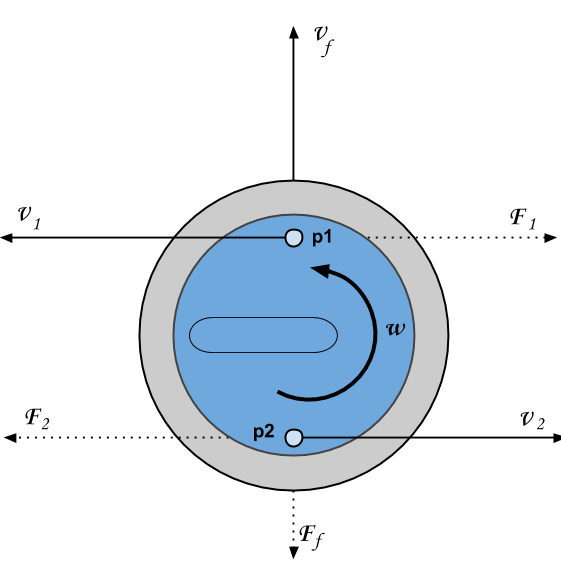
\includegraphics[width=70mm]{Translation.png}
\caption{Påverkan av stenens translation}
\label{fig:Translation}
\label{overflow}
\end{figure}



\subsubsection{Friktionens påverkan}
I kontaktytan mellan isen och curlingstenen uppstår friktion. 
Friktionens påverkan avgörs av stenens kontaktyta samt isens egenskaper. 
Isen påverkas i sin tur av temperatur och luftfuktighet. 
Före spel prepareras isen genom såkallad pebbling då vattendroppar sprids ut över isen och skapar en mindre glatt struktur.
Vid sopning värms isen upp och en tunn vattenhinna skapas framför stenen. Detta gör så att friktion mellan sten och is minskar och därmed går stenen längre vid sopning.  
\\\\Stenens curl beror på att friktionen i den bakre delen \eqref{Fsida2} av stenen är högre än i den främre \eqref{Fsida1}.  
En curlingsten har en kontaktyta mot isen bestående av ett tunt band (ca 5mm brett) som har en något ojämn yta, så kallad scratchad yta. 
När den främre halvan av stenen rör sig över den pebblade isen orsakas ett spår i isen i stenens rörelseriktning med en liten vinkel i rotationsriktningen. 
Då den bakre delen av bandet passerar samma yta ska bandets scratchade yta passera dessa spår, vilka då ligger i nästan rätvinklig riktning från bandets färdriktning, (Figur~\ref{fig:Friktion}). 
Det innebär att den bakre delen av stenen får ett högre motstånd, en högre friktionskraft, än den främre \eqref{biggerthan}
\footnote{H. Nyberg, S. Alfredson, S. Hogmark, S. Jacobson, \emph{The asymmetrical friction mechanism that puts the curl in the curling stone} (2013), Tribomaterials Group, Department of Engineering Sciences, Uppsala University, SE-751 21 Uppsala, Sweden}.
Därmed gör sopning att stenen curlar mindre. Friktionen i punkterna längs bandet påverkas av av stenens rörelse framåt\footnote{A. Raymond Penner, \emph{The physics of sliding cylinders and curling rocks} (2001), American Journal of Physics \textbf{69}, American Association of Physics Teachers},
vilket innebär att friktionskoefficienten $\mu$ påverkas av hastigheten $v$ framåt. Variabeln $c$ är en konstant beroende av friktionspåverkan i punkten. Accelerationen $a$ i en punkt längs stenens band kan därmed beräknas \eqref{mu}.

 \begin{align}\label{Fsida1}
 F_1& = ma_1 = \mu_1 mg \Rightarrow a_1 = \mu_1 g \\\label{Fsida2}
 F_2& = ma_2 = \mu_2 mg \Rightarrow a_2 = \mu_2g \\\label{biggerthan}
 \mu_2& > \mu_1
 \end{align}
\begin{equation}\label{mu} 
\mu = \frac{c}{\sqrt{v}} \Rightarrow a = \frac{cg}{\sqrt{v}} 
\end{equation}

\begin{figure}[ht!]
\centering
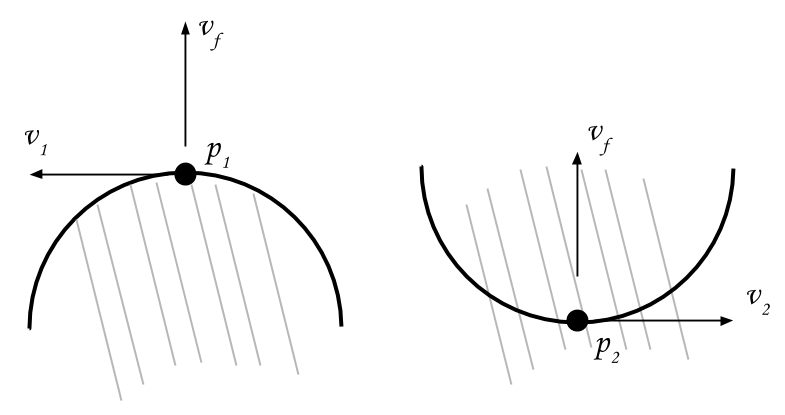
\includegraphics[width=100mm]{Friktion_bakfram.png}
\caption{Friktion i punkt bak respektive fram på stenen. Den bakre delen måste passera de spår framsidan av stenen skapat, vilket leder till högre friktion.}
\label{fig:Friktion}
\label{overflow}
\end{figure}

Den vattenhinna som skapas vid sopning för med sig att de spår som den främre delen av stenen åstadkommer minskar och därmed  även dess effekt på den bakre delen av stenen. 

\subsubsection{Resulterande translation}

Translationen av stenen är en resulterande hastighetsvektor $v$, som består av hastigheten i rörelseriktningen samt av hastigheten i punkterna längs det ringformade band stenen roterar på. Dessa hastigheter kan sammanställas till resultanten i den främre delen av stenen i punkt $p_1$ och den bakre i punkt $p_2$, (Figur~\ref{fig:Translation}). Hastighetens komponenter kan då beskrivas enligt \eqref{vtot}

 \begin{subequations}\label{vtot}
 \begin{align}
 \bar{v_s}& = \bar{v_1}+\bar{v_2}\\
 \bar{v}&=\bar{v_f}+\bar{v_s}
 \end{align}
 \end{subequations}

\subsection{Rotation}


Stenen har även en roterande rörelse med en vinkelhastighet vars ursprungsvärde beräknas utifrån utslagshastigheten av stenen \eqref{vinkelhastighet}.
Vid utslaget antas att spelaren håller stenen så att handtaget pekar i en riktning 90\textdegree  från riktning framåt antingen med inhand eller outhand och släpper stenen med handtaget pekande rakt fram vid hoglinjen. Detta innebär att stenen roterar 90\textdegree under den tid det tar för spelaren att ta sig mellan hack och hog, vilket är direkt kopplat till den angivna utslagshastigheten. 


\begin{align}\label{vinkelhastighet}
 \omega_0 = \frac{\pi}{2 t_0} 
 \end{align}


Friktionen som påverkar rotationshastigheten är summan av all friktion som påverkar bandet som stenen roterar på. Detta kan sammanfattas till friktionen i de två punkterna, $p_1$ och $p_2$ på stenen. Accelerationen på stenens rotation kan därmed beräknas som accelerationen i de två punkterna. 

 \begin{align}\label{a_rotation1}
 \alpha_{rot} =- \frac{( a_1 + a_2)}{r} = -\frac{(\mu_1 g + \mu_2 g)}{r} = - g\frac{c_1+c_2}{r \sqrt{v_f}}
 \end{align}
 
\pagebreak
\subsection{Kollision}

För att kontrollera att en kollision sker beräknas avståndet mellan stenarnas position \eqref{d}.
Om avståndet mellan stenarnas mittpunkter är mindre än två radier \eqref{lessThan} har stenarna krockat  (eftersom krocken bara sker i 2 dimensioner). 

 \begin{subequations}\label{d}
 \begin{align}
 d& = \sqrt{(sten_{1_{xpos}} - sten_{2_{xpos}})^2   +   (sten_{1_{ypos}}-sten_{2_{ypos}})^2}\\\label{lessThan}
 d& \le 2 r
 \end{align}
 \end{subequations}

\begin{figure}[ht!]
\centering
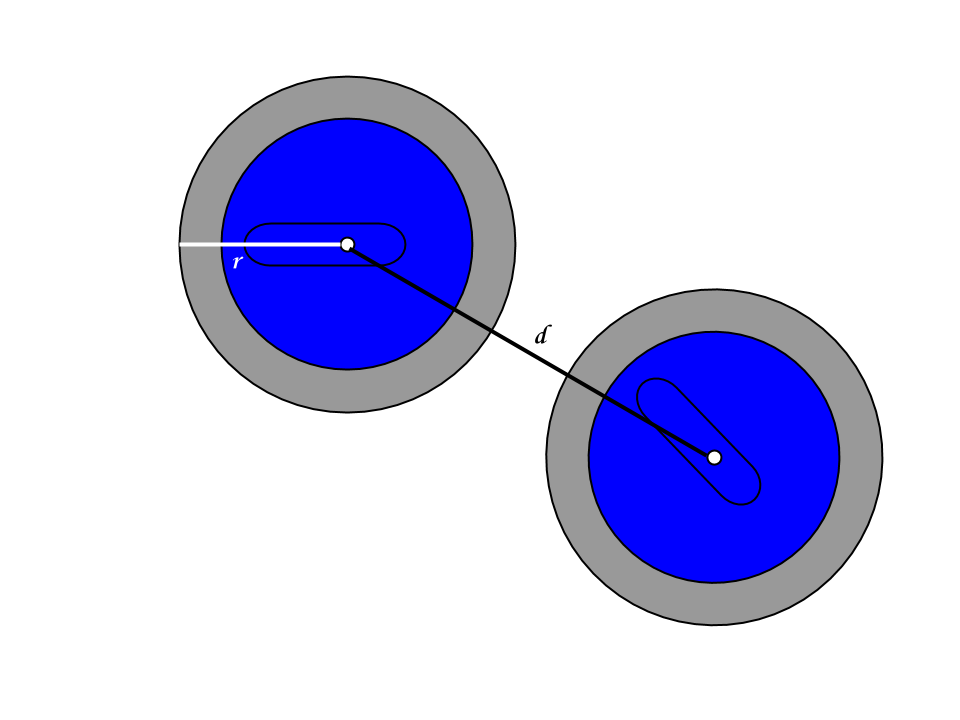
\includegraphics[width=70mm]{krock.png}
\caption{Kontrollera om kollision har inträffat}
\label{fig:kollision}
\label{overflow}
\end{figure}


Hastigheten av curlingstenarna efter en kollision beräknas med hjälp av de två stenarnas position och hastighetsvektorer.
Beräkningarna utgår ifrån en rak central stöt i krockens normalriktning, där det finns två givna ekvationer \eqref{e1} och \eqref{elastisk} för att ta fram hastigheten efter krock.  Dessa ekvationer tar endast hänsyn till fallet då $v’_1 > v’_2$. För att ta det allmäna fallet så måste absolutbeloppet av nämnare och täljaren tas i ekvation \eqref{e1} (vilket kommer leda till två olika fall av ekvation \eqref{vCollision2}  och \eqref{vCollision2n}). 
Med hjälp av stötkoefficienten $e$ \eqref{e1} kan stöten regleras mellan en helt elastikt krock ($e=1$) och en helt inelastiskt krock ($e=0$). 
I curling är det rimligt med en energiförlust och en inelastisk stöt bör därmed tas i beräkning. 
Stötkoefficienten är kvoten av den relativa hastigheten efter kollision och den relativa hastigheten före kollision enligt \eqref{e1}\footnote{R. Grahn, P-Å. Jansson \emph{Dynamik}, Studentlitteratur (1995), s. 334-345}.

Eftersom det ej finns en specificerad stötkoefficient för curlingstenarnas material (granit) har en stötkoefficient uppskattats till 0.3 genom simuleringar.  

 \begin{subequations}\label{e1}
 \begin{align}
 e& = \frac{v_2''-v_1''}{v_1'-v_2'}\\
0& \le e \le 1
 \end{align}
 \end{subequations}
\\\\Oavsett om krocken är inelastisk eller elastisk, gäller lagen om rörelsemängdens bevarande.

 \begin{subequations}\label{elastisk}
 \begin{align}
m_1 v_1' + m_2 v_2'& = m_1 v_1'' + m_2 v_2'' \Rightarrow\\
m_1& = m_2 \Rightarrow\\
v_1' + v_2'& = v_1'' + v_2'' \label{momentum}
 \end{align}
 \end{subequations}


Hastigheterna delas upp i en normal- och tangentkomponent genom att projicera hastighetsvektorn på krocknormalen \eqref{e_normal} och tangentnormalen. Hastighetsvektorn delas upp i dessa komponenter eftersom energiförlusten enbart sker i normalkomponentens riktning. Genom att addera tangentkomponenten med normalkomponenten efter energiförlust, kan sneda krockar hanteras.

 \begin{align}\label{e_normal}
e_n& = \overrightarrow{OP_2} -  \overrightarrow{OP_1}  
 \end{align}

Där $P_1$ och $P_2$ är stenarnas position. Tangentnormalen är ortogonal mot krocknormalen. $e_n$ ses i Figur~\ref{fig:kollision-vektorer}. 

 \begin{align}\label{vCollision}
v_1'& = v_{1n}' + v_{1t}'\\
v_2'& = v_{2n}' + v_{2t}'
 \end{align}

\begin{figure}[ht!]
\centering
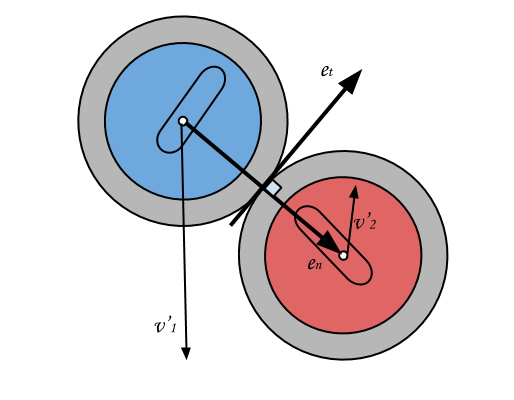
\includegraphics[width=70mm]{kollision-vektorer.png}
\caption{Kollision med riktningar för hastigheter innan krock där $v_{1}$ har högre fart än $v_{2}$}.
\label{fig:kollision-vektorer}
\label{overflow}
\end{figure}

\pagebreak

Kollisionen räknas ut som en rak central stöt med normalkomponenterna, $v_{1n}'$ och  $v_{2n}'$ insatta i ekvation \eqref{e1} och \eqref{momentum}. Hastigheterna efter krocken löses sedan ut, \eqref{vCollision2} och \eqref{vCollision2n}.

 \begin{align}\label{vCollision2}
 v_{1n}''& = \frac{v_{1n}' + v_{2n}'  - e(v_{1n}' + v_{2n}')}{2} \\
 v_{2n}''& = \frac{v_{1n}' + v_{2n}'  + e(v_{1n}' + v_{2n}')}{2} \label{vCollision2n}
 \end{align}


För att få den resulterande hastigheten adderas normalkomponenten efter krock med tangentkomponenten. Illustration hittas i Figur~\ref{fig:efter-krock}. 
 \begin{align}\label{vfinal}
v_1''& = v_{1n}'' + v_{1t}'\\
v_2''& = v_{2n}'' + v_{2t}'
 \end{align}

\begin{figure}[ht!]
\centering
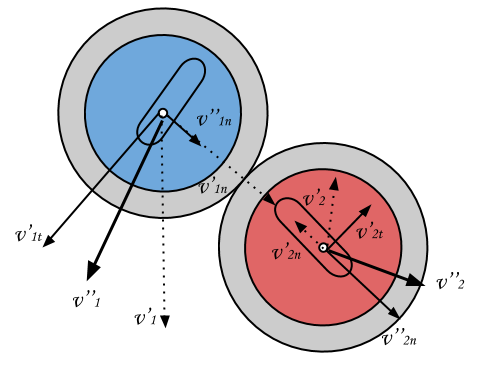
\includegraphics[width=70mm]{efter-krock.png}
\caption{Efter en kollision med normalkomponenterna för hastigheten innan och efter och även den slutgiltiga hastigheten.  }.
\label{fig:efter-krock}
\label{overflow}
\end{figure}


\section{Numeriska metoder för simulering}

\subsection{Numeriska metoder}
Numerisk analys utgår från analytiska uppställningar som kan delas in i stegintervall för
att lösas. Det finns ett flertal algoritmer som använder en numerisk approximation för
att ge en uppskattad men noggrann lösning till svåra problem. Algoritmerna begränsas
av de fel som diskretisering medför och därför får nogrannhet vägas mot beräkningstyngd
när metod väljs. Numeriska algoritmer används ofta inom datorgrafik och simuleringar
för att beräkna till exempel positionen på objekt i rörelse.

\subsubsection{Runge-Kutta-metoden}
Vid lösning av differentialekvationer kan den så kallade Runge-Kutta-metoden användas.
I fallet då differentialekvationen är av första ordningen benämns derivatan av $x$ som en
funktion $f(t, x)$ \eqref{xdot}. Derivatan i den aktuella punkten $x_n$ och efterliggande punkter
beräknas i funktionen $f(t, x)$ med parametrar enligt \eqref{koeff}. Dessa läggs samman för att
beräkna den approximerade funktionsvärdesskillnaden mellan punkterna $x_n$ och $x_{n+1}$.
Den slutliga funktionen \eqref{RungeKutta_transl} beräknar kurvans approximerade värde i nästa steg $x_{n+1}$,
då steglängden har värdet $h$.

 \begin{subequations}
 \begin{align} 
 x_0& = x(t_0)\\ \label{xdot}
 \dot{x}& = f(t,x)
 \end{align}
\end{subequations}

 \begin{subequations}\label{koeff}
 \begin{align}
 k_1& = f(t_0,x_n)\\
 k_2& = f(t_n + frac{1}{2} h, x_n + \frac{h}{2} k_1)\\
 k_3& = f(t_n + frac{1}{2} h, x_n + \frac{h}{2} k_2)\\
 k_4& = f(t_n + h, x_n + h k_3)
 \end{align}
\end{subequations}

 \begin{align}\label{RungeKutta_transl}
 x_{n+1}& =x_n + \frac{h}{6} (k_1+2 k_2 + 2 k_3 + k_4)
 \end{align}

\subsubsection{Eulermetoden}
Eulermetoden är en annan metod för att uppskatta nästa funktionsvärde för en kurva.
Värdet vid efterföljande punkt $x_{n+1}$ är då tidigare punkts funktionsvärde $x_n$ adderat
derivatan i punkten multiplicerat med steglängden $h$ \eqref{euler}.

 \begin{align}\label{euler}
 x_{n+1}& =x_n + \dot{x_n} h
 \end{align}

 \pagebreak

\subsection{Implementation}
För beräkningarna av curlingstenens bana över isen tas hastigheten $v$ fram för varje tid $t$. Hastigheten i den föregående punkten samt den påverkande accelerationen kan i beräkningen behandlas som en differentialekvation av första ordningen. Eftersom positionen för stenen beräknas utifrån hastigheten behöver endast accelerationen med avseende på en variabel (hastigheten i rörelseriktningen) beräknas, $a(v_f)$. Tre farter beräknas i varje steg av simuleringen: fart i rörelseriktningen, fart i ortogonal riktning som tillför curl samt vinkelhastighet. Dessa beräknas genom Runge-Kutta-metoden enligt \eqref{impl}\footnote{L.Ljung, T.Glad \emph{Modellbygge och simulering} (2004), s.380-382}. 

 \begin{subequations}\label{impl}
 \begin{align}
 v_{n+1}& =v_n + \frac{h}{6} (k_1+2 k_2 + 2 k_3 + k_4)\\
 k_1& = a(v_f)\\
 k_2& = a(v_f + \frac{h}{2} k_1)\\
 k_3& = a(v_f + \frac{h}{2} k_2)\\
 k_4& = a(v_f + h k_3)
 \end{align}
\end{subequations}

Funktionen a för accelerationen för de olika farterna olika beroende på de olika friktionstillstånden enligt \eqref{a_front},  \eqref{a_side}, \eqref{a_rotation}\footnote{A. Raymond Penner, \emph{The physics of sliding cylinders and curling rocks} (2001), American Journal of Physics \textbf{69}, American Association of Physics Teachers.}
 
 \begin{align}\label{a_front}
 a_{fram}& = - \mu g\\\label{a_side}
 a_{sida}& = g \frac{c_2-c_1}{\sqrt{v_f}}\\\label{a_rotation}
 a_{rot}& = \alpha_{rot} = - g\frac{c_1+c_2}{r \sqrt{v_f}}
 \end{align}

Samtliga tre parametrar (fart framåt, fart i sidled och vinkelhastighet) är skalärer.
Efter att nästa värde erhållits genom Runge-Kutta-metoden tas hastigheten i riktning
framåt och i sidled fram och de två adderas genom vektoraddition. Ny position av stenen
beräknas i sista steget genom Euler-metoden, där hastighetsvektorn anger riktning och
steglängd \eqref{pos}. 

 \begin{align}\label{pos}
 pos_{n+1}& = pos_{n} + \bar{v} \Delta t
 \end{align}


\section{Grafisk implementering}

\subsection{WebGL}
Efter simuleringen i Matlab har koden skrivits över till WebGL för att avancera det grafiska samt skapa ett spelkoncept på webben. Två spelare kan spela mot varandra och en poängberäkning har implementerats. 

\subsection{Modellering}
Alla objekt, så som stenen och curlingbanan, är modellerade för hand i 3D-grafikprogrammet Blender. På dessa objekt läggs en UV-mappning för att kunna lägga på texturen. Ett konverteringsskript används för att göra om objektet från .obj till .json där UV-koordinaterna blir sparade som strängar. Runtomkring curlingbanan finns en skybox för att skapa illusionen av en stjärnhimmel.

\pagebreak

\section{Resultat}
\subsection{Matlabsimulering}
Valda konstanter för samtliga beräkningar finns i bilaga A, Konstanter och värden. Mått på banan finns i bilaga B. Friktionskonstanter har tagits fram utifrån riktlinjer tagna från referenser där ungefärliga värden beräknats fram genom experiment. De slutgiltiga värdena har tagits fram genom egna undersökningar utifrån de matematiska modellerna för att få fram ett rimligt förhållande mellan utslagshastighet, utslagsvinkel och kurva.   


\begin{figure}[ht!]
\centering
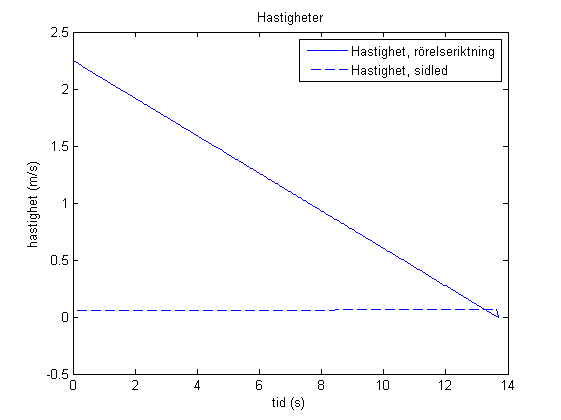
\includegraphics[width=72mm]{hastigheter_tid_graf.png}
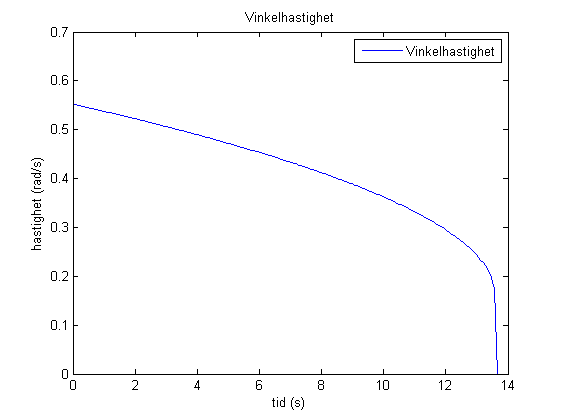
\includegraphics[width=72mm]{vinkelhastighet_tid_graf.png}
\caption{\textbf{t.v} Hastigheter i färdriktning och i sidled som funktion av tid. \textbf{t.h} Vinkelhastighet som funktion av tid}
\label{fig:hast_and_vinkel_graf}
\label{overflow}
\end{figure}


\begin{figure}[ht!]
\centering
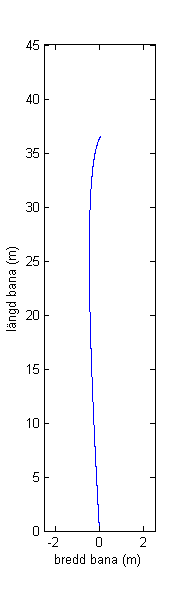
\includegraphics[width=23mm]{curvMatlab.png}
\caption{Hur en curlingstens svängning kan se ut med utslagsvinkeln $3$\textdegree och utslagshastighet $2.3$}
\label{fig:kurvaMatlab}
\label{overflow}
\end{figure}

\pagebreak

\subsection{Grafisk simulering}
Resultatet av projektet blev en curlingsimulering, i form av ett spel, i webbläsaren. Det grafiska gränssnittet ser ut enligt följande: 

\begin{figure}[ht!]
\centering
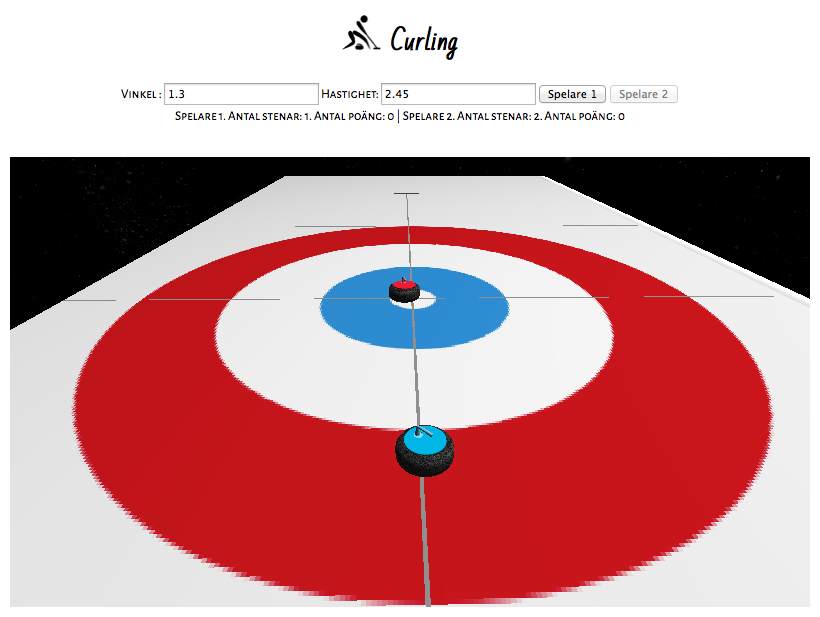
\includegraphics[width=110mm]{game4.png}
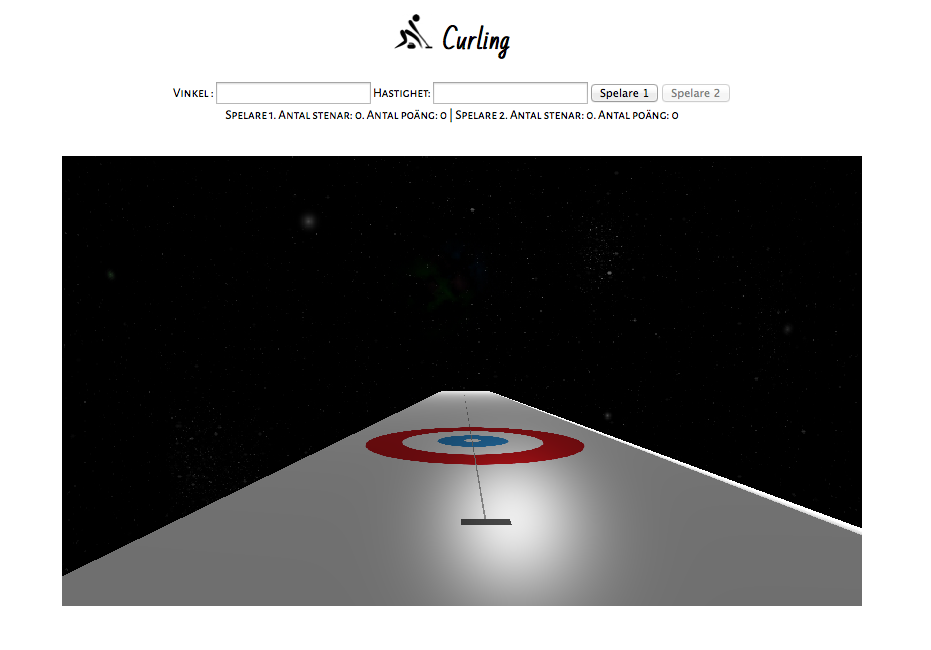
\includegraphics[width=110mm]{game2.png}
\caption{Bilder från spelet}.
\label{fig:spell}
\label{overflow}
\end{figure}


\section{Diskussion}

\subsection{Numeriska metoder}
Vid beräkningarna har två typer av numeriska metoder använts: Eulermetoden och Runge-Kutta-metoden. Runga-Kutta-metoden används vid beräkningen av de nya skalärerna, fart framåt, fart sidled och vinkelhastighet.
Vid implementationen testades både Eulermetoden och Runge-Kutta-metoden. 
För Euler genomfördes beräkningarna med en steglängd på ca. 0.04 sekunder. 
Slutligen valdes Runge-Kutta-metoden då detta gör att beräkningarna blir med noggranna och stabila. 
Däremot har i den visuella simuleringen ingen större skillnad märkts av. Sannolikt beror detta på att Eulermetoden var relativt exakt på grund av den korta steglängden. 
\\\\Vid uträkning av stenens nya position användes Eulermetoden. 
Detta gjordes av två orsaker: positionen beräknas enligt en steglängd längs en vektor i två dimensioner och det är därför implementeringsmässigt enklare och mindre beräkningstungt att använda Euler. 
I annat fall hade vektorn delats upp i flera komponenter och vinningen i det hade varit mindre än problemen som kommer med de tyngre beräkningarna. 

\subsection{Fysik}
Curlingens fysik har varit fokus för ett antal vetenskapliga undersökningar på grund av den speciella sväng (curl) som curlingstenen gör. Det som har förundrat fysikerna är att curlingstenen svänger åt motsatt håll från vad som är standard för andra objekt som kan ses i Figur~\ref{fig:curl}. Teorierna är inte helt överrens varför den svänger som den gör, men en gemensam nämnare är att stenen har en högre friktion bak än fram. Därför har det inte varit helt trivialt hur curlingstenens fysikalsika egenskaper skulle implementeras. Konstanter för exempelvis friktionen fram och bak har inte varit givna i de artiklar som lästs, utan bara relation mellan varandra vilket har givit att vi har testat simuleringen med ett antal olika värden för att komma fram till en så efterliknande sväng som möjligt.

\begin{figure}[ht!]
\centering
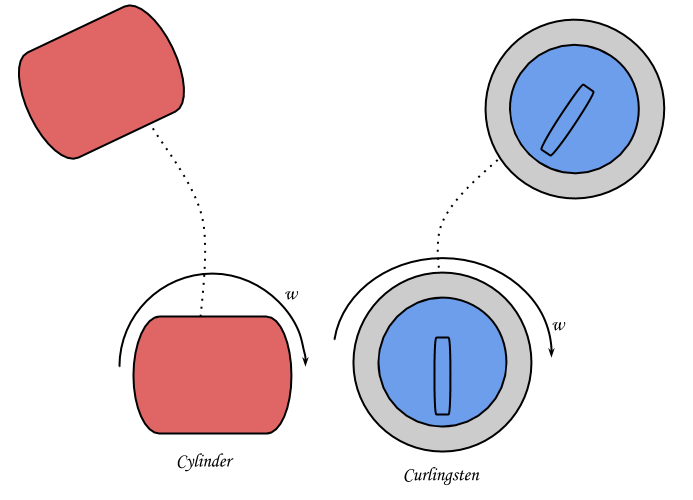
\includegraphics[width=70mm]{curl.png}
\caption{Visar svägningen för en cylinder och en curlingsten. }
\label{fig:curl}
\label{overflow}
\end{figure}

\section{Att köra simuleringen}
Öppna filen index.html i Firefox. Simuleringen fungerar bäst i denna webbläsare då sidan är utvecklad mot Firefox. När sidan är laddad har spelaren möjligheter att röra sig i världen med hjälp av piltangenterna samt tangenterna E och D för att titta upp och ned. Spelare kan själva skjuta iväg en sten genom att bestämma utslagsvinkel och utslagsfart. Det går även att sopa, och därmed minska friktionen, med hjälp av att hålla in tangenten s. Sopningen påverkar enbart den sten som man senast skickade ut för enkelhetens skull. 


\pagebreak
\appendix
\section{\\Konstanter och värden} \label{App:AppendixA}


\begin{tabular}{l | c | r}
benämning & förklaring & värde \\ \hline\hline
\textbf{fysikaliska data} & & \\ \hline
$g$ & gravitationskonstanten & 9.82 $m/s^2$\\
$\mu$ & friktionskonstant & 0.0073\\
$c_1$ & friktionskonstant fram & 0.000001\\
$c_2$ & friktionskonstant bak & 0.0001\\
\textbf{curlingstenen} & & \\ \hline
$m$ & massa & 18 kg\\
$r$ & radie sten & 0.1454676 m\\
$r_{inner}$ & radie kontaktband & 0.06 m\\ \hline
\end{tabular}

\section{\\Mått och bild på curlingstenens bana} \label{App:AppendixB}

\begin{figure}[ht!]
\centering
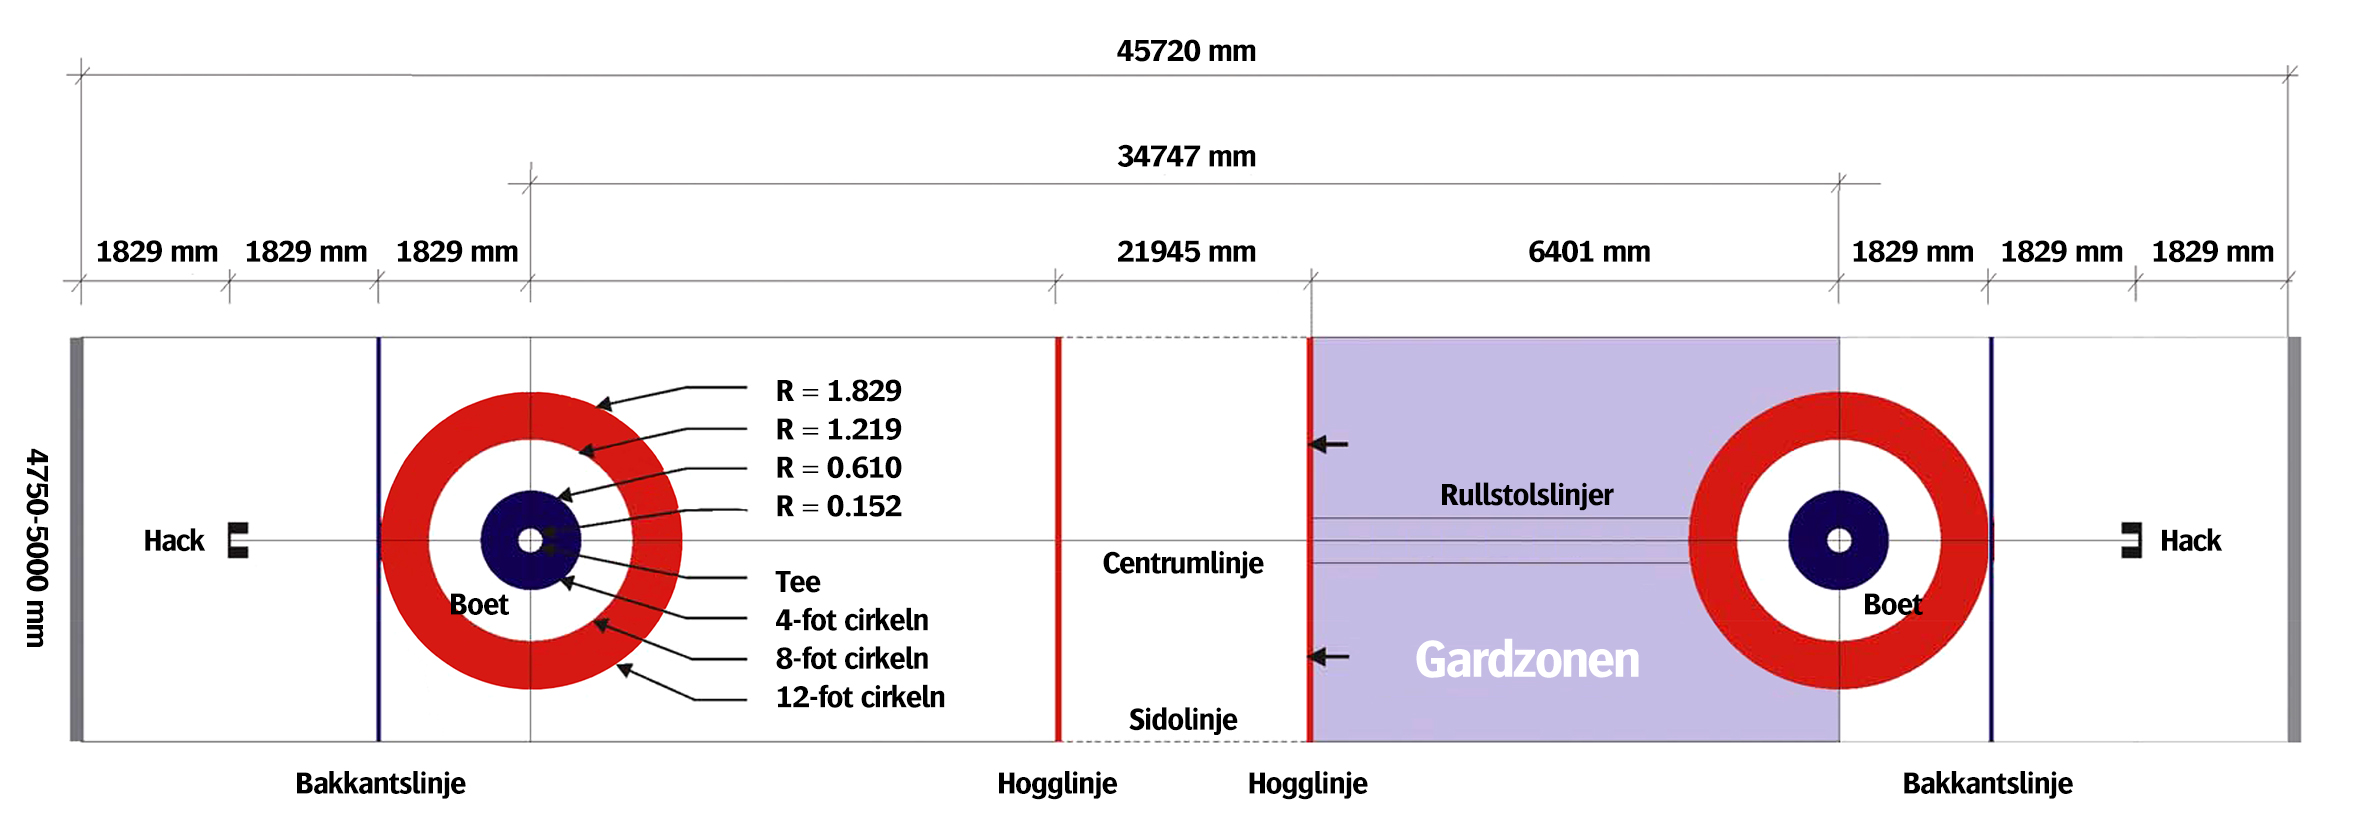
\includegraphics[width=160mm]{curlingbana.jpg}
\caption{Mått på en curlingbana}
\label{fig:curlbana_riktigt}
\label{overflow}
\end{figure}




\end{document}
